\documentclass{standalone}
\usepackage{tikz}
\usetikzlibrary{patterns, positioning}


\begin{document}
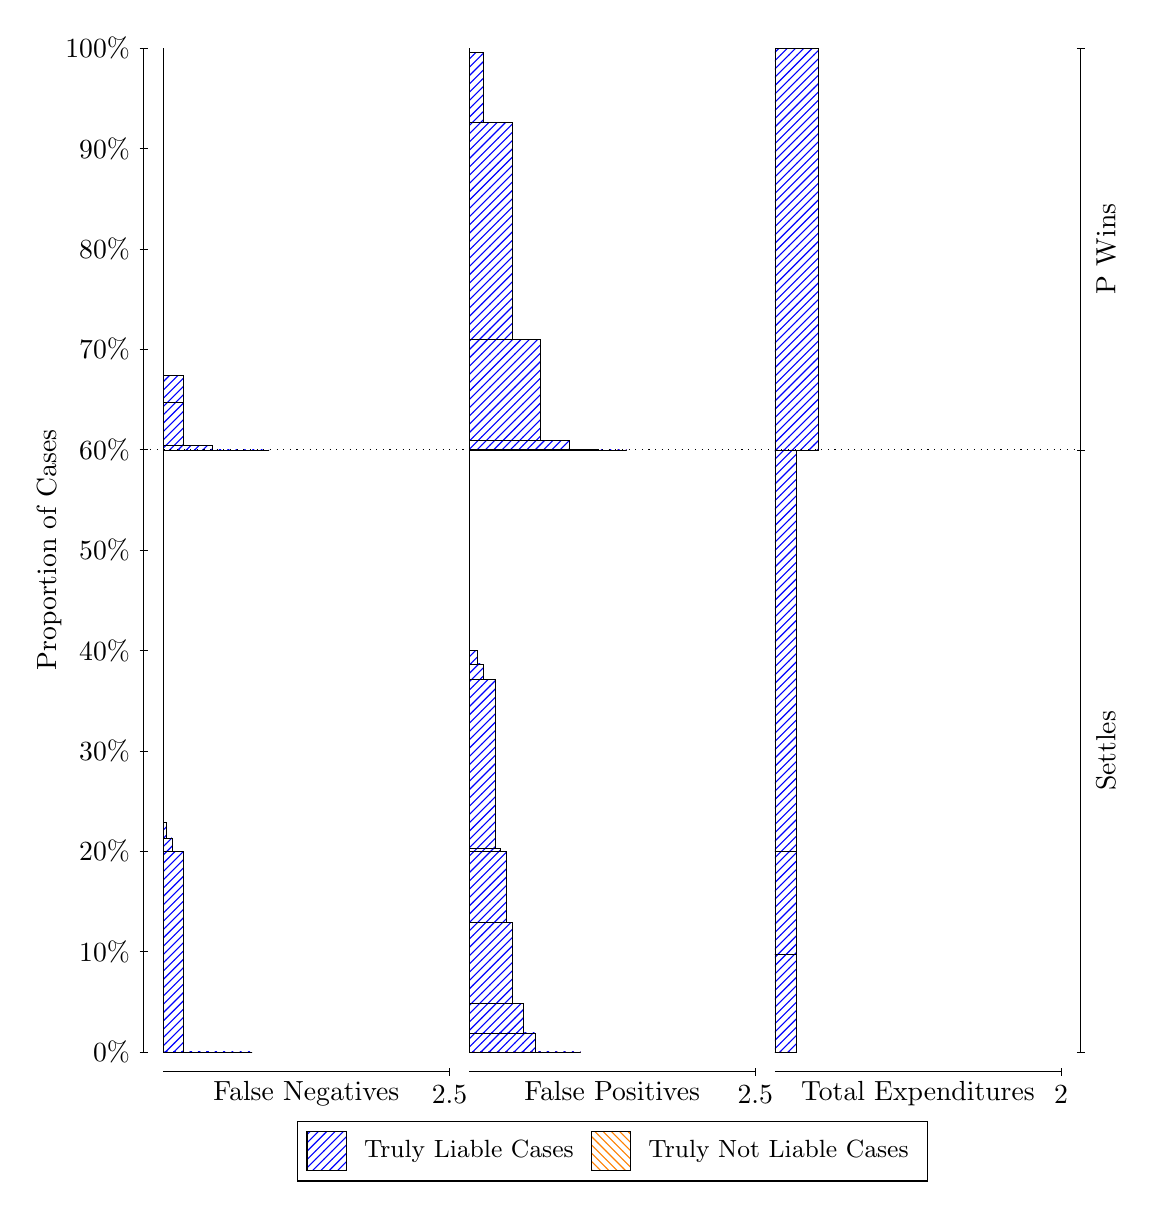
\begin{tikzpicture}
\draw[black, very thin] (1.5,1.75) -- (1.5,14.5);
\node[rotate=90, text=black, anchor=center] at (0.3, 8.125) {Proportion of Cases};
\draw[black, very thin] (1.45,1.75) -- (1.55,1.75);
\node[text=black, anchor=east] at (1.45, 1.75) {0\%};
\draw[black, very thin] (1.45,3.025) -- (1.55,3.025);
\node[text=black, anchor=east] at (1.45, 3.025) {10\%};
\draw[black, very thin] (1.45,4.3) -- (1.55,4.3);
\node[text=black, anchor=east] at (1.45, 4.3) {20\%};
\draw[black, very thin] (1.45,5.575) -- (1.55,5.575);
\node[text=black, anchor=east] at (1.45, 5.575) {30\%};
\draw[black, very thin] (1.45,6.85) -- (1.55,6.85);
\node[text=black, anchor=east] at (1.45, 6.85) {40\%};
\draw[black, very thin] (1.45,8.125) -- (1.55,8.125);
\node[text=black, anchor=east] at (1.45, 8.125) {50\%};
\draw[black, very thin] (1.45,9.4) -- (1.55,9.4);
\node[text=black, anchor=east] at (1.45, 9.4) {60\%};
\draw[black, very thin] (1.45,10.675) -- (1.55,10.675);
\node[text=black, anchor=east] at (1.45, 10.675) {70\%};
\draw[black, very thin] (1.45,11.95) -- (1.55,11.95);
\node[text=black, anchor=east] at (1.45, 11.95) {80\%};
\draw[black, very thin] (1.45,13.225) -- (1.55,13.225);
\node[text=black, anchor=east] at (1.45, 13.225) {90\%};
\draw[black, very thin] (1.45,14.5) -- (1.55,14.5);
\node[text=black, anchor=east] at (1.45, 14.5) {100\%};

\draw[black, very thin] (13.4,1.75) -- (13.4,14.5);
\draw[black, very thin] (13.35,1.75) -- (13.45,1.75);
\node[anchor=west] at (13.35, 1.75) {};
\draw[black, very thin] (13.35,9.3977) -- (13.45,9.3977);
\node[anchor=west] at (13.35, 9.3977) {};
\draw[black, very thin] (13.35,14.5) -- (13.45,14.5);
\node[anchor=west] at (13.35, 14.5) {};

\draw[black, very thin, pattern color=blue, pattern=north east lines] (1.75,1.75) rectangle (2.8763,1.75);
\draw[black, very thin, pattern color=blue, pattern=north east lines] (1.75,1.75) rectangle (2.5857,1.75);
\draw[black, very thin, pattern color=blue, pattern=north east lines] (1.75,1.75) rectangle (2.513,1.75);
\draw[black, very thin, pattern color=blue, pattern=north east lines] (1.75,1.75) rectangle (2.4403,1.75);
\draw[black, very thin, pattern color=blue, pattern=north east lines] (1.75,1.75) rectangle (2.295,1.75);
\draw[black, very thin, pattern color=blue, pattern=north east lines] (1.75,1.75) rectangle (2.2223,1.7503);
\draw[black, very thin, pattern color=blue, pattern=north east lines] (1.75,1.7503) rectangle (2.1497,1.7517);
\draw[black, very thin, pattern color=blue, pattern=north east lines] (1.75,1.7517) rectangle (2.077,1.7517);
\draw[black, very thin, pattern color=blue, pattern=north east lines] (1.75,1.7517) rectangle (2.0043,4.2976);
\draw[black, very thin, pattern color=blue, pattern=north east lines] (1.75,4.2976) rectangle (1.9317,4.299);
\draw[black, very thin, pattern color=blue, pattern=north east lines] (1.75,4.299) rectangle (1.859,4.4689);
\draw[black, very thin, pattern color=blue, pattern=north east lines] (1.75,4.4689) rectangle (1.7863,4.6695);
\draw[black, very thin, pattern color=orange, pattern=north west lines] (1.75,4.6695) rectangle (1.75,4.6695);
\draw[black, very thin, pattern color=blue, pattern=north east lines] (1.75,4.6695) rectangle (1.75,9.3977);
\draw[black, very thin, pattern color=blue, pattern=north east lines] (1.75,9.3977) rectangle (3.0943,9.3977);
\draw[black, very thin, pattern color=blue, pattern=north east lines] (1.75,9.3977) rectangle (2.731,9.3978);
\draw[black, very thin, pattern color=blue, pattern=north east lines] (1.75,9.3978) rectangle (2.3677,9.4513);
\draw[black, very thin, pattern color=blue, pattern=north east lines] (1.75,9.4513) rectangle (2.0043,10.002);
\draw[black, very thin, pattern color=blue, pattern=north east lines] (1.75,10.002) rectangle (2.0043,10.341);
\draw[black, very thin, pattern color=orange, pattern=north west lines] (1.75,10.341) rectangle (1.75,10.341);
\draw[black, very thin, pattern color=blue, pattern=north east lines] (1.75,10.341) rectangle (1.75,14.5);
\draw[black, very thin, pattern color=orange, pattern=north west lines] (5.6333,1.75) rectangle (7.0503,1.75);
\draw[black, very thin, pattern color=blue, pattern=north east lines] (5.6333,1.75) rectangle (7.0503,1.75);
\draw[black, very thin, pattern color=orange, pattern=north west lines] (5.6333,1.75) rectangle (6.7597,1.75);
\draw[black, very thin, pattern color=blue, pattern=north east lines] (5.6333,1.75) rectangle (6.7597,1.75);
\draw[black, very thin, pattern color=blue, pattern=north east lines] (5.6333,1.75) rectangle (6.687,1.7517);
\draw[black, very thin, pattern color=orange, pattern=north west lines] (5.6333,1.7517) rectangle (6.6143,1.7517);
\draw[black, very thin, pattern color=blue, pattern=north east lines] (5.6333,1.7517) rectangle (6.6143,1.7517);
\draw[black, very thin, pattern color=orange, pattern=north west lines] (5.6333,1.7517) rectangle (6.469,1.7517);
\draw[black, very thin, pattern color=blue, pattern=north east lines] (5.6333,1.7517) rectangle (6.469,1.9918);
\draw[black, very thin, pattern color=blue, pattern=north east lines] (5.6333,1.9918) rectangle (6.3963,1.9932);
\draw[black, very thin, pattern color=blue, pattern=north east lines] (5.6333,1.9932) rectangle (6.3237,2.3654);
\draw[black, very thin, pattern color=blue, pattern=north east lines] (5.6333,2.3654) rectangle (6.251,2.3657);
\draw[black, very thin, pattern color=orange, pattern=north west lines] (5.6333,2.3657) rectangle (6.1783,2.3657);
\draw[black, very thin, pattern color=blue, pattern=north east lines] (5.6333,2.3657) rectangle (6.1783,3.4003);
\draw[black, very thin, pattern color=blue, pattern=north east lines] (5.6333,3.4003) rectangle (6.1057,4.3023);
\draw[black, very thin, pattern color=blue, pattern=north east lines] (5.6333,4.3023) rectangle (6.033,4.3344);
\draw[black, very thin, pattern color=blue, pattern=north east lines] (5.6333,4.3344) rectangle (5.9603,6.4779);
\draw[black, very thin, pattern color=blue, pattern=north east lines] (5.6333,6.4779) rectangle (5.8877,6.4782);
\draw[black, very thin, pattern color=blue, pattern=north east lines] (5.6333,6.4782) rectangle (5.815,6.6787);
\draw[black, very thin, pattern color=blue, pattern=north east lines] (5.6333,6.6787) rectangle (5.7423,6.8487);
\draw[black, very thin, pattern color=blue, pattern=north east lines] (5.6333,6.8487) rectangle (5.6697,6.8501);
\draw[black, very thin, pattern color=blue, pattern=north east lines] (5.6333,6.8501) rectangle (5.6333,9.3977);
\draw[black, very thin, pattern color=orange, pattern=north west lines] (5.6333,9.3977) rectangle (7.6317,9.3977);
\draw[black, very thin, pattern color=blue, pattern=north east lines] (5.6333,9.3977) rectangle (7.6317,9.3977);
\draw[black, very thin, pattern color=orange, pattern=north west lines] (5.6333,9.3977) rectangle (7.2683,9.3977);
\draw[black, very thin, pattern color=blue, pattern=north east lines] (5.6333,9.3977) rectangle (7.2683,9.399);
\draw[black, very thin, pattern color=orange, pattern=north west lines] (5.6333,9.399) rectangle (6.905,9.399);
\draw[black, very thin, pattern color=blue, pattern=north east lines] (5.6333,9.399) rectangle (6.905,9.5142);
\draw[black, very thin, pattern color=orange, pattern=north west lines] (5.6333,9.5142) rectangle (6.5417,9.5142);
\draw[black, very thin, pattern color=blue, pattern=north east lines] (5.6333,9.5142) rectangle (6.5417,10.795);
\draw[black, very thin, pattern color=orange, pattern=north west lines] (5.6333,10.795) rectangle (6.1783,10.795);
\draw[black, very thin, pattern color=blue, pattern=north east lines] (5.6333,10.795) rectangle (6.1783,13.557);
\draw[black, very thin, pattern color=blue, pattern=north east lines] (5.6333,13.557) rectangle (5.815,14.446);
\draw[black, very thin, pattern color=blue, pattern=north east lines] (5.6333,14.446) rectangle (5.6333,14.5);
\draw[black, very thin, pattern color=orange, pattern=north west lines] (9.5167,1.75) rectangle (9.7892,1.75);
\draw[black, very thin, pattern color=blue, pattern=north east lines] (9.5167,1.75) rectangle (9.7892,2.9866);
\draw[black, very thin, pattern color=orange, pattern=north west lines] (9.5167,2.9866) rectangle (9.7892,2.9866);
\draw[black, very thin, pattern color=blue, pattern=north east lines] (9.5167,2.9866) rectangle (9.7892,4.2989);
\draw[black, very thin, pattern color=orange, pattern=north west lines] (9.5167,4.2989) rectangle (9.7892,4.2989);
\draw[black, very thin, pattern color=blue, pattern=north east lines] (9.5167,4.2989) rectangle (9.7892,9.3977);
\draw[black, very thin, pattern color=orange, pattern=north west lines] (9.5167,9.3977) rectangle (10.062,9.3977);
\draw[black, very thin, pattern color=blue, pattern=north east lines] (9.5167,9.3977) rectangle (10.062,14.5);
\draw[black, dotted] (1.5,9.3977) -- (13.4,9.3977);
\draw[black, very thin] (1.75,1.5) -- (5.3833,1.5);
\node[text=black, anchor=north] at (3.5667, 1.5) {False Negatives};
\draw[black, very thin] (5.3833,1.45) -- (5.3833,1.55);
\node[text=black, anchor=north] at (5.3833, 1.45) {2.5};

\draw[black, very thin] (5.6333,1.5) -- (9.2667,1.5);
\node[text=black, anchor=north] at (7.45, 1.5) {False Positives};
\draw[black, very thin] (9.2667,1.45) -- (9.2667,1.55);
\node[text=black, anchor=north] at (9.2667, 1.45) {2.5};

\draw[black, very thin] (9.5167,1.5) -- (13.15,1.5);
\node[text=black, anchor=north] at (11.333, 1.5) {Total Expenditures};
\draw[black, very thin] (13.15,1.45) -- (13.15,1.55);
\node[text=black, anchor=north] at (13.15, 1.45) {2};

\node[text=black, centered, rotate=90] at (13.72, 5.5738) {Settles};
\node[text=black, centered, rotate=90] at (13.72, 11.949) {P Wins};

\draw (7.449999999999999,1.5) node[draw=none] (baseCoordinate) {};
\begin{scope}[align=center]
        \matrix[scale=0.5, draw=black, below=0.5cm of baseCoordinate, nodes={draw}, column sep=0.1cm]{
            \node[rectangle, draw, minimum width=0.5cm, minimum height=0.5cm, pattern color=blue, pattern=north east lines] {}; &
            \node[draw=none, font=\small, text=black] (B) {Truly Liable Cases}; &
            \node[rectangle, draw, minimum width=0.5cm, minimum height=0.5cm, pattern color=orange, pattern=north west lines] {}; &
            \node[draw=none, font=\small, text=black] (B) {Truly Not Liable Cases}; \\
            };
\end{scope}

\end{tikzpicture}
\end{document}